\documentclass[11pt]{article}
\usepackage{geometry}
\geometry{margin=1in}
\usepackage{graphicx}
\usepackage{amsmath}
\usepackage{listings}
\usepackage{hyperref}
\usepackage{tikz}
\usetikzlibrary{shapes.geometric, arrows.meta, positioning}
\tikzstyle{startstop} = [rectangle, rounded corners, minimum width=3cm, minimum height=1cm,text centered, draw=black, fill=gray!20]
\tikzstyle{process} = [rectangle, minimum width=3cm, minimum height=1cm, text centered, draw=black, fill=blue!10]
\tikzstyle{decision} = [diamond, minimum width=3.5cm, minimum height=1cm, text centered, draw=black, fill=orange!20]
\tikzstyle{arrow} = [thick,->,>=stealth]


\title{Cache Simulator Report}
\author{}
\date{}

\begin{document}

\maketitle

\section{Implementation Details}

The cache simulator has been implemented in C++ using a modular and object-oriented approach. The main components are:

\subsection*{1. Main Driver: \texttt{main.cpp}}
This file initializes the simulation environment and drives the application by:
\begin{itemize}
  \item Reading configuration and trace files.
  \item Instantiating cache controllers.
  \item Managing the simulation loop.
\end{itemize}

\subsection*{2. Cache Access: \texttt{cacheAccess.cpp/h}}
This module defines the logic to access individual cache blocks, perform tag checks, determine hit/miss, and handle block replacements using LRU policies.

\subsection*{3. Cache Controller: \texttt{cacheController.cpp/h}}
Handles operations at the level of the whole cache:
\begin{itemize}
  \item Coordinates between memory requests and cache responses.
  \item Implements cache coherence if necessary.
  \item Maintains statistics (hits, misses, execution time).
\end{itemize}

\subsection*{4. Cache Structures: \texttt{cacheStructure.h}}
Defines the internal data representation of cache blocks and sets. Important structures include:
\begin{itemize}
  \item \texttt{CacheBlock} with tag, valid/dirty bits.
  \item \texttt{CacheSet} with a list/vector of blocks, supporting LRU management.
\end{itemize}

\subsection*{5. Bus Operation: \texttt{busOperation.cpp/h}}
Responsible for coordinating memory access across processors:
\begin{itemize}
  \item Emulates memory bus or interconnect.
  \item Synchronizes memory operations (loads/stores).
\end{itemize}

\subsection*{6. Configuration: \texttt{cacheconf.h}}
Defines simulation parameters such as:
\begin{itemize}
  \item Cache size (default: 4KB).
  \item Associativity (default: 2-way).
  \item Block size (default: 32 bytes).
\end{itemize}

\section*{Flowchart of Cache Simulation}

\begin{center}
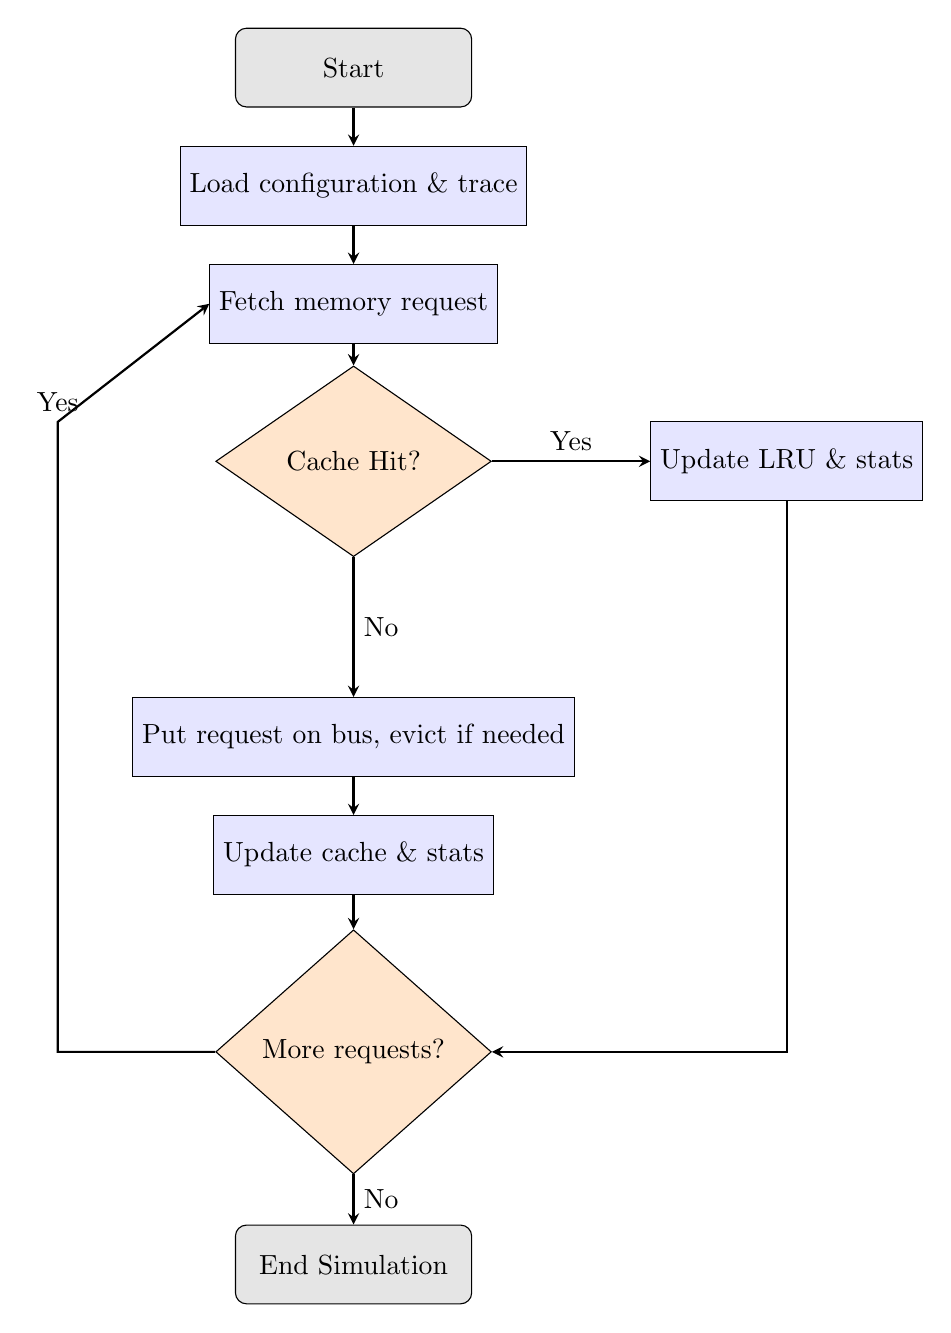
\begin{tikzpicture}[node distance=1.5cm]

\node (start) [startstop] {Start};
\node (load) [process, below of=start] {Load configuration \& trace};
\node (request) [process, below of=load] {Fetch memory request};
\node (check) [decision, below of=request, yshift=-0.5cm] {Cache Hit?};
\node (hit) [process, right of=check, xshift=4cm] {Update LRU \& stats};
\node (miss) [process, below of=check, yshift=-2cm] {Put request on bus, evict if needed};
\node (update) [process, below of=miss] {Update cache \& stats};
\node (more) [decision, below of=update, yshift=-1.0cm] {More requests?};
\node (end) [startstop, below of=more, yshift=-1.2cm] {End Simulation};

\draw [arrow] (start) -- (load);
\draw [arrow] (load) -- (request);
\draw [arrow] (request) -- (check);
\draw [arrow] (check) -- node[above] {Yes} (hit);
\draw [arrow] (hit) |- (more);
\draw [arrow] (check) -- node[right] {No} (miss);
\draw [arrow] (miss) -- (update);
\draw [arrow] (update) -- (more);
\draw [arrow] (more) -- node[right] {No} (end);
\draw [arrow] (more.west) -- ++(-2,0) -- ++(0,8) node[above] {Yes} -- (request.west);


\end{tikzpicture}
\end{center}

\section{Cache Coherence}
To ensure consistent memory views across the four L1 caches in our quad-core simulator, we implemented cache coherence using the MESI protocol within a bus-based snooping architecture. The following outlines the coherence model and detailed behavior under different memory access cases.

\begin{itemize}
  \item \textbf{Bus-Based Snooping:} Each cache monitors a shared global bus for memory operations initiated by other processors. This allows each cache to snoop and respond to relevant transactions to maintain coherence.

  \item \textbf{Write Invalidate Protocol:} We adopt a write-invalidate approach, where a processor writing to a cache line broadcasts an invalidate message, causing other caches to invalidate their copies. This significantly reduces bus bandwidth usage compared to write-update schemes, particularly for high-write traffic scenarios.

  \item \textbf{MESI States:}
    \begin{itemize}
      \item \textbf{Modified (M):} Cache line is only in the local cache and has been modified.
      \item \textbf{Exclusive (E):} Cache line is clean and held exclusively by one cache.
      \item \textbf{Shared (S):} Cache line is clean and may exist in multiple caches.
      \item \textbf{Invalid (I):} Cache line is invalid or out-of-date.
    \end{itemize}

  \item \textbf{Assumptions of MESI protocol followed}
    \begin{itemize}
      \item \textbf{Read Hit:}
        \begin{itemize}
          \item No bus activity is triggered.
          \item Data is simply returned from the local cache.
          \item State remains unchanged (must be in M, E, or S).
          \item In all the cases only 1 cycle wil be require as we are directly getting hits in the L1 cache.
        \end{itemize}

      \item \textbf{Read Miss:} 
        \begin{itemize}
          \item Bus read is issued. Action depends on other cache states:
          \begin{itemize}
            \item \emph{No copies elsewhere:} Data is read from memory and stored with state \textbf{E}.(100 cycles of memory penalty)
            \item \emph{One copy in E:} That cache supplies data over the bus(cache to cache transfer); both change to \textbf{S}.(2*N cycles of transfer penalty)
            \item \emph{Copies in S:} One cache supplies data(cache to cache transfer); all caches including requester stay in \textbf{S}.(2*N cycles of tranfer penalty)
            \item \emph{Copy in M:} M cache writes back data to memory and shares it on the bus(cache to cache transfer); source transitions M $\rightarrow$ S, requester gets \textbf{S}.(100 cycles of cache penalty + 2*N cycles of tranfer penalty)
            \item In all the above cases a additional 1 cycle will be required for cache access.
          \end{itemize}
        \end{itemize}

      \item \textbf{Write Hit:} 
        \begin{itemize}
          \item \emph{M state:} Line is already dirty. Update value, no state change.(1 cycle for direct hit)
          \item \emph{E state:} Line is clean and private. Update value, state changes to \textbf{M}.(1 cycle for direct hit)
          \item \emph{S state:} Broadcast invalidate. Other caches with S copy move to \textbf{I}. Update local value, local state becomes \textbf{M}.(1 cycle for hit ,we are doing invalidation in same cycleas the miss happened at local cache)
        \end{itemize}

      \item \textbf{Write Miss:}
        \begin{itemize}
          \item Bus transaction issued as RWITM (Read With Intent To Modify).
          \item Depending on copies in other caches:
          \begin{itemize}
            \item \emph{No copies:} Data is read from memory, updated, and marked (100 cycles for memory access)\textbf{M}.
            \item \emph{Copies in S or E:} Invalidate broadcast forces others to \textbf{I}. Local line is updated and marked \textbf{M}.(100 cycles for memory access)
            \item \emph{Copy in M:} The owner (in M) delays RWITM, writes back to memory, and invalidates its line. Then the requester retries RWITM, updates its line, and sets it to \textbf{M}.(100 cyles for writing copy to memory and 100 cycles again for reading value from memory into local cache)
          \end{itemize}
        \end{itemize}
    \end{itemize}

  \item \textbf{Remote Processor Accesses (Snooped Events)}
    \begin{itemize}
      \item \textbf{Mem Read:}
        \begin{itemize}
          \item Caches with line in E, S, or M may respond.
          \item M state cache writes back value, transitions to \textbf{S}.
          \item E or S caches stay in \textbf{S}.
        \end{itemize}
      \item \textbf{RWITM (Write Miss):}
        \begin{itemize}
          \item All caches holding the line invalidate their copy (S or E $\rightarrow$ I).
          \item M cache must write back and then invalidate (M $\rightarrow$ I).
        \end{itemize}
      \item \textbf{Invalidate:}
        \begin{itemize}
          \item All caches matching the address invalidate their line.
        \end{itemize}
    \end{itemize}

  \item \textbf{Write-Back Support:} In contrast to write-through caches, we use write-back policy. Modified lines are written to memory only on eviction, reducing bus traffic and improving performance.

\end{itemize}



\section{Assumptions and Interpretations}
\subsection*{1. Bus arbitration}
The bus arbitration is assumed as follows:Ties are broken arbitrarily on the bus as is done in real systems when multiple cores attempt bus transactions simultaneously.The operating system's thread scheduler determines which waiting thread gets the bus access when multiple cores try to access it(we started the project earlier so we have taken this assumption as was written originally in the pdf) So we were able to obtain different data across simulation which we could analyse properly.


\subsection*{2. Bus Transactions}
Only one active bus transaction can happen at any time, including memory
fetches, cache-to-cache transfers, and invalidates. Local Cache hit 1 cycles,
if its miss the request gets placed on bus, we are doing invalidation/RDx/WRX also in same cycle
as the miss happened at local cache.


\section{Definitions}

\subsection*{1. Core Statistics}

Based on the implementation in the source code, the following statistics are tracked and calculated for each core:

\subsubsection*{2. Total Instructions}
The total number of memory access operations (reads and writes) processed by the cache controller. Each memory access from the trace file increments \texttt{totalInstructions} counter in the \texttt{cacheController.cpp} after the \texttt{cacheAccess} function completes execution.

\subsubsection*{3. Total Reads}
A counter that specifically tracks read operations. This is incremented in the \texttt{runTracefile} method when a line starting with "R" is encountered in the trace file, and also updated in \texttt{cacheAccess} when \texttt{isWrite} is false.

\subsubsection*{4. Total Writes}
Calculated as the difference between total instructions and total reads: \texttt{totalInstructions - totalReads}. This represents all write operations processed by the cache.

\subsubsection*{5. Total Execution Cycles}
The \texttt{globalCycles} counter counts cycles spent executing its own instruction trace.
\begin{itemize}
  \item Cache access: Always adds \texttt{config.cacheAccessCycles} (100 cycles)
  \item Cache misses: Adds additional memory access cycles
  \item Bus operations: Adds cycles depending on operations like invalidations and state transitions
  \item MESI transitions: Different state changes have different cycle penalties
\end{itemize}

\subsubsection*{6. Idle Cycles}
Idle cycles are cycles spent waiting for the resources while other cores
are executing its instructions.Once a core finishes executing all its instructions, it is considered done.
Further cycles are not counted under idle cycles for that core.

\subsubsection*{7. Cache Misses}
The \texttt{globalMisses} counter is incremented in \texttt{cacheAccess} when \texttt{response->hit} is 0, indicating either:
\begin{itemize}
  \item The tag wasn't found in the cache
  \item The block was found but marked invalid
\end{itemize}

\subsubsection*{8. Cache Miss Rate}
Calculated as \texttt{(globalMisses / totalInstructions) * 100}, giving a percentage of how often memory accesses missed the cache.

\subsubsection*{9. Cache Evictions}
The \texttt{globalEvictions} counter tracks when existing blocks must be removed to make room for new blocks. This is incremented in \texttt{cacheAccess} when \texttt{response->eviction} is not 0.

\subsubsection*{10. Writebacks}
\begin{itemize}
  \item Writebacks are incremeted whenever any cache writes back to memory nothing else is added in writebacks.
\end{itemize}
The total of a core represents all memory writes from a cache to main memory.

\subsubsection*{11. Bus Invalidations}
The \texttt{busInvalidations} counter is incremented in \texttt{busOperation.cpp} when another core forces this core to invalidate a cache line through bus signaling. This happens when:
\begin{itemize}
  \item Another core writes to a shared line
  \item Cache coherence protocol requires invalidation for consistency
\end{itemize}

\subsubsection*{12. Data Traffic (Bytes)}
The \texttt{dataTrafficBytes} counter represents memory bandwidth usage, incremented by \texttt{blockSize} when:
\begin{itemize}
  \item Cache misses occur (reading from memory)
  \item Dirty evictions occur (writing back to memory)
  \item Cache-to-cache transfers occur (particularly for shared data)
  \item MESI transitions that require data movement
\end{itemize}

\subsection*{13. Overall Bus Summary}

\subsubsection*{a. Total Bus Transactions}
Represents the total number of operations that occurred on the bus across all cores.

\subsubsection*{b. Total Bus Traffic (Bytes)}
The sum of \texttt{dataTrafficBytes} from all cores, representing the total amount of data transferred over the bus during the simulation.

\section{Experimental Results}
To understand the behavior and consistency of our cache simulator, we conducted multiple experimental runs with identical parameters. Each experiment used the default configuration of a 4KB 2-way set associative L1 cache per processor with 32-byte block size. The simulator was run 10 times with the same application input, and the results were collected to analyze the variability in performance metrics.

\subsection{Simulation Parameters}
\begin{itemize}
  \item \textbf{Cache Size:} 4KB per processor
  \item \textbf{Associativity:} 2-way set associative
  \item \textbf{Block Size:} 32 bytes
  \item \textbf{Number of Cores:} 4
  \item \textbf{Number of Simulation Runs:} 10
\end{itemize}

\subsection{Variation in Execution Cycles}
Figure \ref{fig:exec_cycles} shows the distribution of execution cycles across all 10 runs for each of the four cores.

\begin{figure}[h]
  \centering
  \includegraphics[width=0.8\textwidth]{chart.png}
  \caption{Execution Cycles Distribution Across 10 Runs for Each Core}
  \label{fig:exec_cycles}
\end{figure}

The execution cycles data reveals several important observations:

\begin{itemize}
  \item \textbf{Core-specific Patterns:} Core 2 consistently requires significantly more execution cycles (approximately 3.51 million) compared to the other cores, which average between 3.0-3.05 million cycles. This indicates that Core 2 is likely executing more memory-intensive operations or experiencing more complex memory access patterns.
  
  \item \textbf{Run-to-Run Variation:} Despite identical input parameters, we observe minor variations in execution cycles across different runs. For example, Core 0's execution cycles range from approximately 3,044,417 to 3,058,073 cycles, showing a variation of about 0.45\%.
  
  \item \textbf{Relative Consistency:} While absolute cycle counts vary, the relative performance between cores remains consistent across runs, with Core 2 always requiring the most cycles, followed typically by Core 0, then Core 3, and Core 1 generally being the most efficient.
\end{itemize}

\subsection{Analysis of Cache Miss Rates}
Figure \ref{fig:miss_rates} illustrates the miss rates for each core across all 10 simulation runs.

\begin{figure}[h]
  \centering
  \includegraphics[width=0.8\textwidth]{chart1.png}
  \caption{Cache Miss Rate Distribution Across 10 Runs for Each Core}
  \label{fig:miss_rates}
\end{figure}

The miss rate data reveals interesting patterns:

\begin{itemize}
  \item \textbf{Remarkable Stability:} Unlike execution cycles, miss rates demonstrate exceptional stability across different runs for each individual core. For instance, Core 0's miss rate remains within the narrow range of 1.53715\% to 1.53751\%.
  
  \item \textbf{Core-specific Miss Behaviors:} Core 2 consistently shows the highest miss rate (approximately 1.733\%), which aligns with its higher execution cycle count. Meanwhile, Core 1 exhibits the lowest miss rate (approximately 1.518\%), explaining its generally lower execution cycles.
  
  \item \textbf{Correlation with Performance:} The hierarchy of miss rates (Core 2 > Core 0 > Core 3 > Core 1) strongly correlates with the general pattern observed in execution cycles, confirming that cache performance is a dominant factor in overall execution efficiency.
\end{itemize}


\section{Cache Parameter Impact Analysis}
To investigate the performance impact of different cache parameters, we extended the simulator to compute maximum execution time across all cores for various cache configurations. We systematically varied three key parameters (cache size, associativity, and block size) from the default configuration to three alternative values in powers of 2, keeping other parameters constant during each analysis.

\subsection{Impact of Number of Sets}
Figure \ref{fig:num_sets} illustrates the maximum execution time across cores as we vary the number of cache sets from 32 to 128, effectively changing the cache size while keeping associativity and block size constant.

\begin{figure}[h]
  \centering
  \includegraphics[width=0.8\textwidth]{vary_sets_analysis.png}
  \caption{Maximum Execution Time vs. Number of Sets}
  \label{fig:num_sets}
\end{figure}

As the number of sets increases from 32 to 128 (effectively increasing cache size from 2KB to 8KB with constant associativity of 2 and block size of 32 bytes), we observe a dramatic reduction in execution time. The most significant improvement occurs when doubling the sets from 32 to 64, yielding a 23.08\% reduction in execution cycles. Further doubling to 128 sets provides an additional improvement, but with diminishing returns, reaching a total reduction of 31.10\% compared to the baseline.

This behavior can be attributed to a significant reduction in conflict misses as addresses are distributed across more sets. The diminishing returns at higher set counts suggest that beyond a certain point, the workload's working set fits more comfortably in the cache, and remaining misses are likely compulsory or capacity misses rather than conflict misses.

\subsection{Impact of Associativity}
Figure \ref{fig:associativity} shows how maximum execution time changes as we increase associativity from 2-way to 8-way, keeping the number of sets and block size constant.

\begin{figure}[h]
  \centering
  \includegraphics[width=0.8\textwidth]{vary_associativity_analysis.png}
  \caption{Maximum Execution Time vs. Associativity}
  \label{fig:associativity}
\end{figure}

Increasing associativity from 2-way to 4-way yields a substantial 10.07\% improvement in execution time. However, further increasing to 8-way provides only a marginal additional benefit of about 1.26\%, for a total improvement of 11.33\% compared to the baseline.

This pattern indicates that the workload experiences a significant number of conflict misses that can be mitigated by increasing associativity from 2 to 4. The minimal additional gain from 4-way to 8-way suggests that after 4-way, most conflict misses have been eliminated, and remaining misses are likely compulsory or capacity misses that cannot be addressed by increasing associativity alone.

\subsection{Impact of Block Size}
Figure \ref{fig:block_size} demonstrates the effect of varying block size from 16 bytes to 64 bytes on maximum execution time.

\begin{figure}[h]
  \centering
  \includegraphics[width=0.8\textwidth]{vary_block_size_analysis.png}
  \caption{Maximum Execution Time vs. Block Size}
  \label{fig:block_size}
\end{figure}

The block size experiments reveal a more complex relationship with performance. Increasing block size from 16 bytes to 32 bytes results in a substantial 22.24\% reduction in execution time, indicating strong spatial locality in the workload. However, further increasing to 64 bytes causes performance to degrade slightly, with execution time increasing by 4.68\% compared to the 32-byte configuration.

This non-monotonic behavior suggests an interesting tradeoff: while larger blocks can better exploit spatial locality by prefetching nearby data, excessively large blocks can lead to cache pollution and increased miss penalties when spatial locality is not uniformly strong. The 32-byte block size appears optimal for this workload, balancing the benefits of prefetching against the costs of transferring unnecessarily large blocks.

\subsection{Overall Parameter Impact Analysis}
Comparing across all three parameters, we observe that:

\begin{itemize}
  \item \textbf{Number of sets} (effectively cache size) has the largest overall impact, with a maximum improvement of 31.10\% when increased from 32 to 128 sets.
  
  \item \textbf{Block size} shows the second largest impact but with an optimal point at 32 bytes, demonstrating a 22.24\% improvement over 16 bytes.
  
  \item \textbf{Associativity} provides more modest but still significant benefits of 11.33\% when increased from 2-way to 8-way.
\end{itemize}

The optimal cache configuration for this workload appears to be 128 sets with 4-way associativity and 32-byte blocks. This configuration strikes a good balance between reducing conflict misses through increased associativity and sets while optimizing for the workload's spatial locality characteristics with an appropriate block size.

These findings emphasize the importance of tuning cache parameters to specific workload characteristics, as each parameter affects different types of cache misses. For this particular application, increasing the number of sets (effectively the cache size) provides the most substantial performance benefit, suggesting that the working set size is a primary factor limiting performance.

\end{document}
